\section{ Linear regression with one variable }

\subsection{ Plotting the Data}

\begin{itemize}
    \item How many features are involved in this problem?
    \subitem We have one feature (population of a city) and one target variable (profit of a food truck). 
    \item How much data is involved in this problem?
    \subitem We have 97 data points (97 cities) in the dataset.
    \item What is the problem from a machine learning point-of-view?
    \subitem Supervised/Unsupervised?
    \subitem Supervised learning, as we have input-output pairs (population-profit).
    \subitem Regression/Classification?
    \subitem Regression, as we are predicting a continuous value (profit) based on the input feature (population).
    \subitem Linear/?on-linear problem
    \subitem Linear problem, as we are trying to fit a linear model to the data. 
\end{itemize}

\begin{figure}[H]
    \centering
    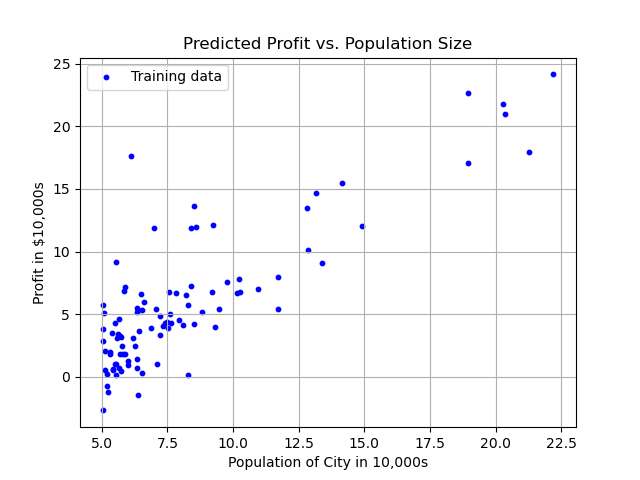
\includegraphics[width=0.75\linewidth]{figure/base_datas.png}
    \label{fig:placeholder}
\end{figure}

\section{Gradient Descent}
\subsection{Computing the cost J($\theta$)}

\begin{lstlisting}
import numpy as np

def computeCost(X, y, theta):  
    """
       computes the cost of using theta as the parameter for linear 
       regression to fit the data points in X and y
    """
    m = y.size
    J = 0.

    # =============YOUR CODE HERE ===============
    # Instructions: Compute the cost of a particular choice of theta


    #h = float(theta[0,0]) + float(theta[1,0])*X[:,1]
    #h = h.reshape((m,1))
    h = X @ theta
    J = (1/(2*m)) * np.sum((h-y)**2)
    
	#   ===========================================

    return J
\end{lstlisting}

\subsection{Gradient descent}

\begin{lstlisting}
import numpy as np
from computeCost import computeCost

def gradientDescent(X, y, theta, alpha, num_iters):  
    """
     Performs gradient descent to learn theta
       theta, cost_history, theta_history = gradientDescent(X, y, theta, alpha, num_iters) updates theta by
       taking num_iters gradient steps with learning rate alpha
    """
    # Initialize some useful values
    m = y.size  # number of training examples
    n = theta.size # number of parameters
    cost_history = np.zeros(num_iters) # cost over iters
    theta_history = np.zeros((n,num_iters)) # theta over iters

    for i in range(num_iters):
    #   ====================== YOUR CODE HERE ======================
    # Instructions: Perform a single gradient step on the parameter vector
    #               theta.
    #
    # Hint: While debugging, it can be useful to print out the values
    #       of the cost function (computeCost) and gradient here.

        h = X @ theta

        theta[0,0] = theta[0,0] - (alpha/m)*np.sum( ((h-y)*X[:,0].reshape((m,1)))  )  
        theta[1,0] = theta[1,0] - (alpha/m)*np.sum(((h-y)*X[:,1].reshape((m,1))))

        cost_history[i] = computeCost(X, y, theta)
        theta_history[:,i] = theta.reshape((2,))
    
    #   =====================================

    return theta, cost_history, theta_history
\end{lstlisting}

In this part, we can see the datas (X and y) are constant. However, the parameters (theta) are updated at each iteration of the gradient descent algorithm. The cost function J($\theta$) is computed at each iteration to monitor the convergence of the algorithm. The goal is at each interation to update the parameters (theta) in the direction that reduces the cost function more quicly possible to the global minimum. 

Training data with linear regression fit :

\begin{figure}[H]
    \centering
    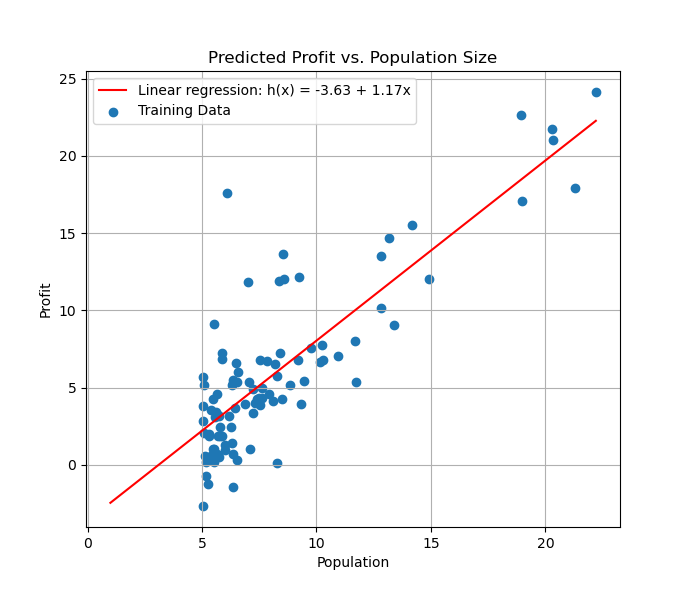
\includegraphics[width=0.75\linewidth]{figure/linear_regr.png}
    \label{fig:placeholder}
\end{figure}

\subsection{Visualizing J($\theta$)}

\begin{figure}[H]
    \centering
    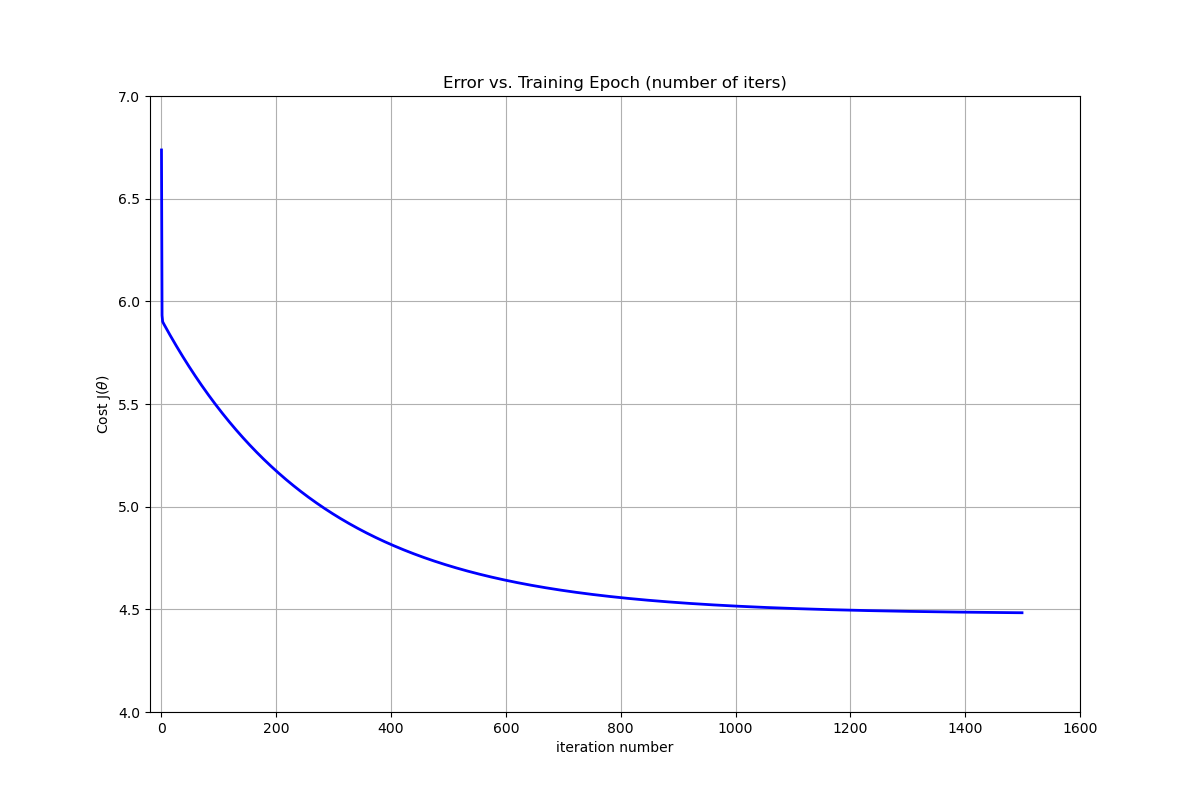
\includegraphics[width=0.75\linewidth]{figure/cost_f.png}
    \label{fig:placeholder}
\end{figure}

In this part, we can see the cost function J($\theta$) is a convex function, which means it has a single global minimum. The contour plot shows the values of J($\theta$) for different values of $\theta_0$ and $\theta_1$. The red dot represents the optimal parameters (theta) that minimize the cost function. 

\begin{figure}[H]
    \centering
    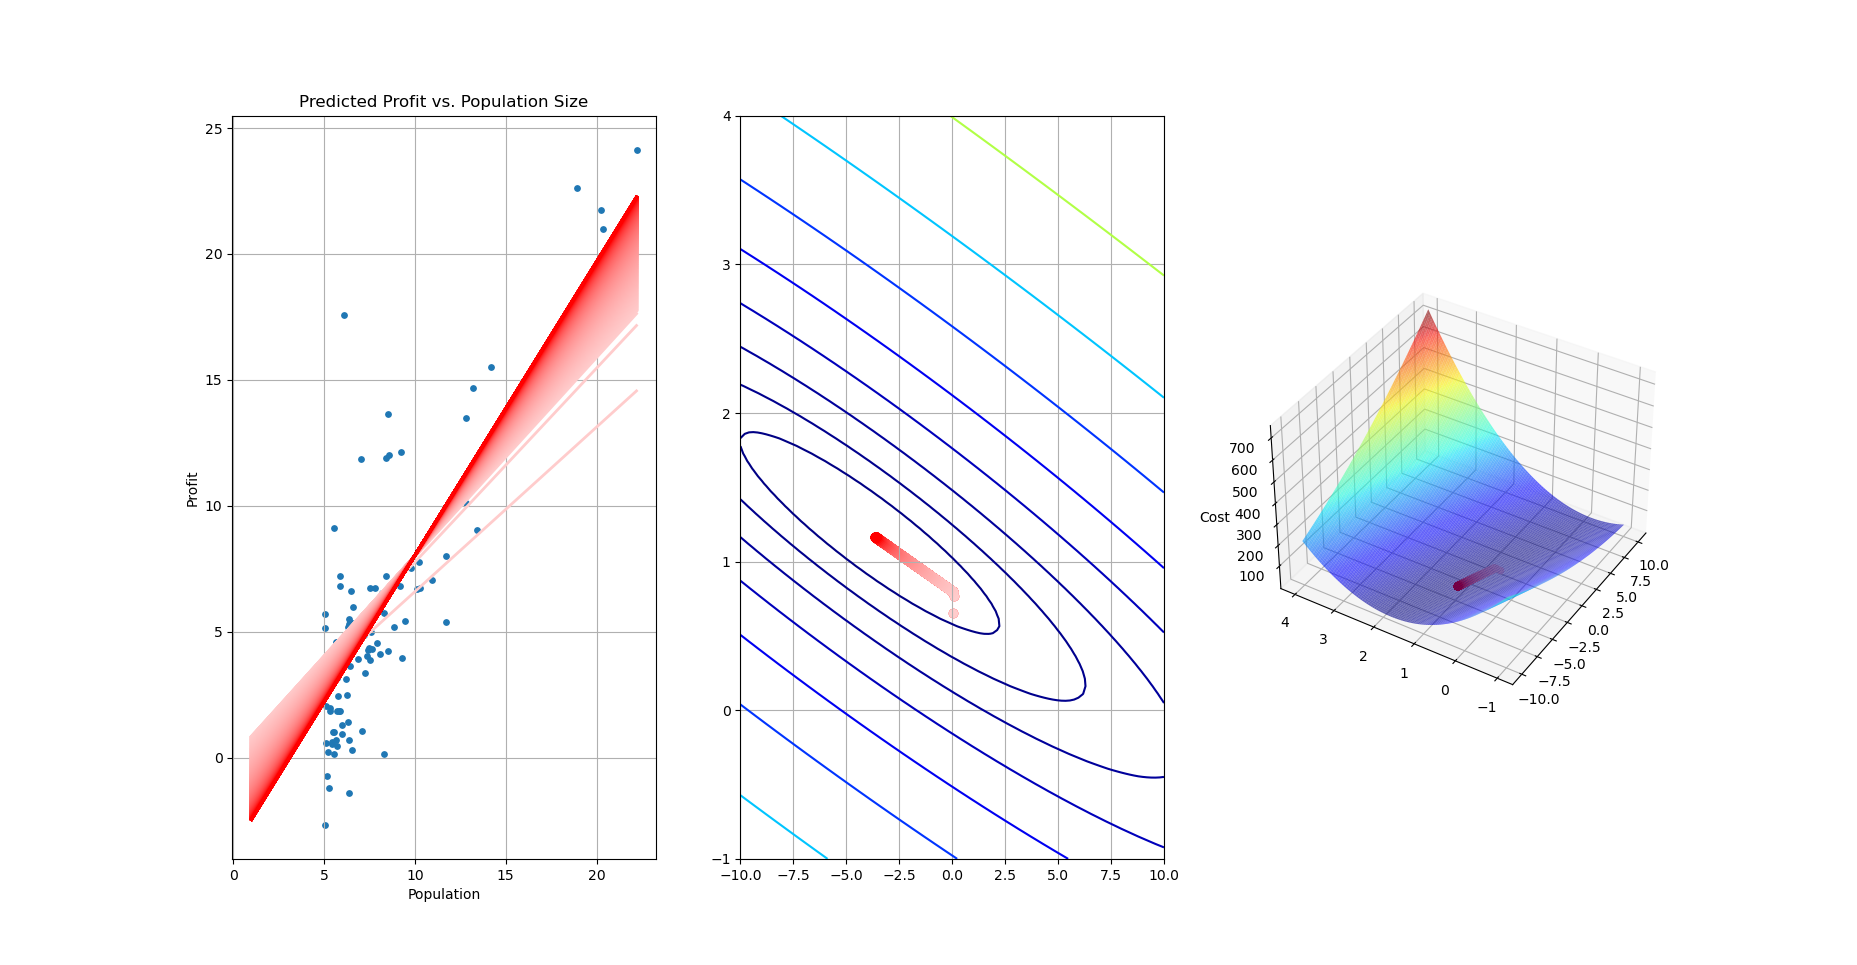
\includegraphics[width=0.75\linewidth]{figure/cost_2.png}
    \label{fig:placeholder}
\end{figure}

\section{Linear regression with multiple variables}
\subsection{Feature Normalization}

\begin{lstlisting}
import numpy as np


def featureNormalize(X):
    """
       returns a normalized version of X where
       the mean value of each feature is 0 and the standard deviation
       is 1. This is often a good preprocessing step to do when
       working with learning algorithms.
    """
    X_norm, mu, sigma = 0,0,0
    # ====================== YOUR CODE HERE ======================
    # Instructions: First, for each feature dimension, compute the mean
    #               of the feature and subtract it from the dataset,
    #               storing the mean value in mu. Next, compute the
    #               standard deviation of each feature and divide
    #               each feature by it's standard deviation, storing
    #               the standard deviation in sigma.
    #
    #               Note that X is a matrix where each column is a
    #               feature and each row is an example. You need
    #               to perform the normalization separately for
    #               each feature.
    #
    # Hint: You might find the 'mean' and 'std' functions useful.
    #


    mu = np.mean(X, axis=0)
    sigma = np.std(X, axis=0)
    X_norm = (X - mu) / sigma



	# =========================================

    return X_norm, mu, sigma
\end{lstlisting}

\subsection{Learning with gradient descent}
\subsubsection{ Compute cost and gradients}


\begin{lstlisting}
import numpy as np
from computeCostMulti import computeCostMulti

def gradientDescentMulti(X, y, theta, alpha, num_iters):  
    """
     Performs gradient descent to learn theta
       theta = gradientDescent(x, y, theta, alpha, num_iters) updates theta by
       taking num_iters gradient steps with learning rate alpha
    """
    # Initialize some useful values
    m = y.size  # number of training examples
    n = theta.size # number of parameters
    cost_history = np.zeros(num_iters)
    theta_history = np.zeros((n,num_iters))

    for i in range(num_iters):
    #   ====================== YOUR CODE HERE ======================
    # Instructions: Perform a single gradient step on the parameter vector
    #               theta.
    #
    # Hint: While debugging, it can be useful to print out the values
    #       of the cost function (computeCost) and gradient here.
    #

        h = X @ theta
        grad = (1/m) * (X.T @ (h - y))
        theta = theta - alpha * grad

        cost_history[i] = computeCostMulti(X, y, theta)
        theta_history[:,i] = theta.reshape((n,))
      
    #   =================================================
        
    return theta, cost_history, theta_history
\end{lstlisting}

\begin{figure}[H]
    \centering
    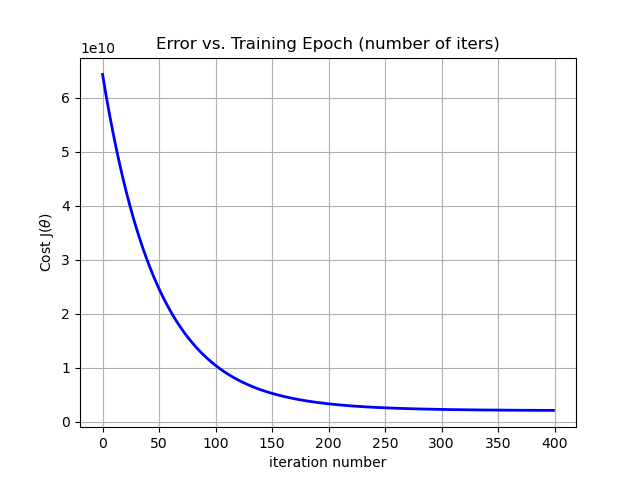
\includegraphics[width=0.75\linewidth]{figure/j_mult_1.png}
    \label{fig:placeholder}
\end{figure}

\subsubsection{Selecting learning rates}

\begin{figure}[H]
    \centering
    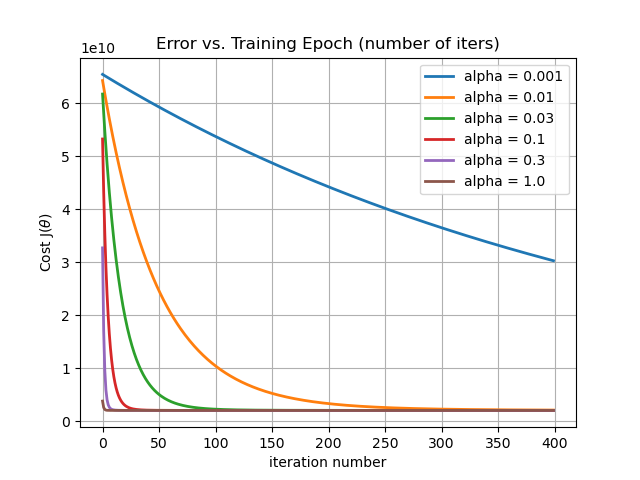
\includegraphics[width=0.75\linewidth]{figure/j_alpha.png}
    \label{fig:placeholder}
\end{figure}

The range of valeus for the learning rate $\alpha$ was between 0.001 and 1.0 if the we passed of 1.0 the cost function J($\theta$) diverged and the algorithm did not converge to the global minimum. The best learning rate was 1.0, as it converged faster to the global minimum than the other learning rates.

\subsubsection{Predict the price for a new house}

\begin{lstlisting}
import numpy as np

# Estimate the price of a 1650 sq-ft, 3 br house
def predict_multi(house_features, mu, sigma, theta):

    #   ====================== YOUR CODE HERE ======================
    # You should use the learned model with its characteristics (mu, sigma, theta)
    # to predict the price of a house based on its features (surface and bedrooms)

    house_features_norm = (house_features-mu)/sigma
    house_features_norm = np.concatenate((np.ones((1, 1)), house_features_norm), axis=1)
    price = house_features_norm.dot(theta)
    print(f'shapes {np.shape(theta)}  {np.shape(house_features_norm)}')
    return price
\end{lstlisting}

\begin{itemize}
    \item Predicted price of a 1650 sq-ft, 3 br house
(using gradient descent): 293081.4643349
\end{itemize}


\begin{figure}[H]
    \centering
    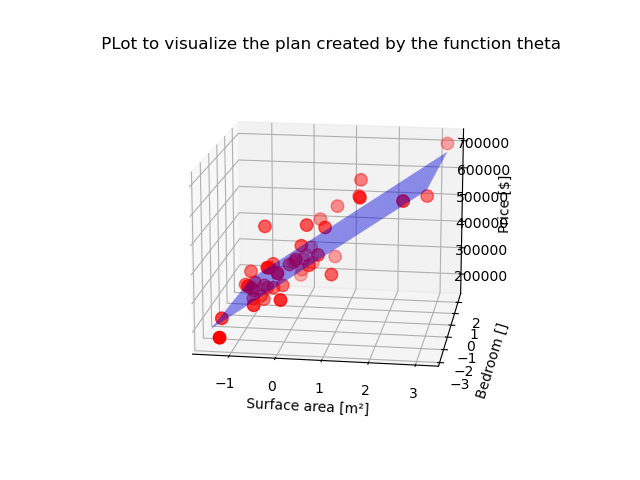
\includegraphics[width=0.75\linewidth]{figure/plan.png}
    \label{fig:placeholder}
\end{figure}

\subsection{ Optional exercise: Normal Equations}

\begin{lstlisting}
import numpy as np


def normalEqn(X,y):
   """ Computes the closed-form solution to linear regression
      normalEqn(X,y) computes the closed-form solution to linear
      regression using the normal equations.
   """


   # ====================== YOUR CODE HERE ======================
   # Instructions: Complete the code to compute the closed form solution
   #               to linear regression and put the result in theta.
   #

   t = np.linalg.pinv(X.T @ X) @ X.T @ y


   # ===================================================

   return t

\end{lstlisting}

Solving with normal equations...

Theta computed from the normal equations:
 [[89597.90954355]
 [  139.21067402]
 [-8738.01911255]] 

\begin{itemize}
    \item Predicted price of a 1650 sq-ft, 3 br house 
(using normal equations):
293081.464335
\end{itemize}

We can see that the predicted price of a 1650 sq-ft, 3 br house is very close using gradient descent and normal equations. The normal equations method is more efficient for small datasets, while gradient descent is more efficient for large datasets.

\subsection{ Some questions, you have to answer...}

\begin{itemize}
    \item Définissez les termes :
    \subitem  Approches supervisées/non-supervisées
    \subitem Apprentissage supervisé : l’algorithme apprend à partir d’exemples étiquetés (input-output pairs) pour prédire la sortie pour de nouvelles entrées. Apprentissage non-supervisé : l’algorithme apprend à partir de données non étiquetées pour trouver des structures ou des motifs dans les données.

    \subitem Régression/ Classification
    \subitem Régression : On utilise ça quand on veut deviner un chiffre précis (comme le prix d'une maison ou une température). Classification : On utilise ça quand on veut deviner une catégorie (par exemple, dire si une image montre un chat ou un chien).

    \subitem Descripteurs/features
    \subitem Ce sont les informations qu'on utilise pour faire notre choix. Pour notre exercice, c'est la taille de la maison et le nombre de chambres.
    \subitem Cibles
    \subitem C'est le résultat qu'on veut deviner. Ici, c'est le prix de la maison.
    \subitem Modèle de régression linéaire
    \subitem C'est une idée mathématique qui dit que les informations et le résultat sont liés par une ligne droite. Si la maison est plus grande, le prix monte de façon régulière.



    \item Représenter en un schéma général, les processus d’apprentissage et de prédiction.
    
\textbf{L'apprentissage (créer le modèle) :}
\begin{itemize}
    \item[] Données connues (Descripteurs + Cibles)
    \item[$\rightarrow$] L'ordinateur s'entraîne et corrige ses erreurs
    \item[$\rightarrow$] On obtient un modèle prêt.
\end{itemize}

\vspace{0.5cm}

\textbf{La prédiction (utiliser le modèle) :}
\begin{itemize}
    \item[] Nouvelles données (Descripteurs d'une nouvelle maison, sans le prix)
    \item[$\rightarrow$] Le modèle fait son calcul
    \item[$\rightarrow$] Il nous donne le prix deviné.
\end{itemize}











    \item Comment fonctionne l’apprentissage? Par quels moyens? A quoi sert la fonction de coût? Comment
est-résolu le problème? Connaissez vous d’autres moyens de le résoudre?
    \subitem Comment ça marche ? Au début, le modèle devine le prix un peu au hasard. Ensuite, il regarde s'il a fait une grosse erreur ou pas. Il change un peu ses réglages pour être meilleur la prochaine fois. Il fait ça des centaines de fois.

À quoi sert la fonction de coût ? C'est comme une note qui mesure les erreurs du modèle. Le but de l'algorithme est d'avoir l'erreur la plus petite possible.

Comment le problème est résolu ? On a utilisé la méthode de la descente de gradient. C'est une technique où l'ordinateur avance petit à petit pour descendre vers l'erreur la plus petite.

D'autres moyens de le résoudre ? Oui, on a aussi programmé l'équation normale. C'est un grand calcul mathématique qui trouve la meilleure réponse d'un seul coup, sans avancer pas à pas.
    \item Pourquoi faut-il parfois normaliser les descripteurs (features)?
    \subitem On fait ça quand on a des données avec des chiffres très différents. Par exemple, la taille de la maison est très grande (1650) et le nombre de chambres est très petit (3). L'algorithme a du mal à comparer ces choses et ça ralentit beaucoup les calculs.
Normaliser, c'est transformer ces chiffres pour les mettre sur la même échelle (par exemple, tout mettre entre -1 et 1). Grâce à ça, le programme trouve la solution beaucoup plus vite.
\end{itemize}